% !TEX TS-program = pdflatex
% !TEX encoding = UTF-8 Unicode

% This is a simple template for a LaTeX document using the "article" class.
% See "book", "report", "letter" for other types of document.

\documentclass[11pt]{article} % use larger type; default would be 10pt
\usepackage[svgnames]{xcolor}
\usepackage{listings}
\lstset{language=R,
    basicstyle=\small\ttfamily,
    stringstyle=\color{DarkGreen},
    otherkeywords={0,1,2,3,4,5,6,7,8,9},
    morekeywords={TRUE,FALSE},
    deletekeywords={data,frame,length,as,character},
    keywordstyle=\color{blue},
    commentstyle=\color{DarkGreen},
}
\usepackage{amsmath}
\usepackage[backend=biber]{biblatex}
\usepackage[utf8]{inputenc} % set input encoding (not needed with XeLaTeX)
\usepackage{listings}
\usepackage{amsmath}
%%% Examples of Article customizations
% These packages are optional, depending whether you want the features they provide.
% See the LaTeX Companion or other references for full information.

%%% PAGE DIMENSIONS
\usepackage{geometry} % to change the page dimensions
\geometry{a4paper} % or letterpaper (US) or a5paper or....
% \geometry{margin=2in} % for example, change the margins to 2 inches all round
% \geometry{landscape} % set up the page for landscape
%   read geometry.pdf for detailed page layout information

\usepackage{graphicx} % support the \includegraphics command and options

% \usepackage[parfill]{parskip} % Activate to begin paragraphs with an empty line rather than an indent

%%% PACKAGES
\usepackage{booktabs} % for much better looking tables
\usepackage{array} % for better arrays (eg matrices) in maths
\usepackage{paralist} % very flexible & customisable lists (eg. enumerate/itemize, etc.)
\usepackage{verbatim} % adds environment for commenting out blocks of text & for better verbatim
\usepackage{subfig} % make it possible to include more than one captioned figure/table in a single float
% These packages are all incorporated in the memoir class to one degree or another...

%%% HEADERS & FOOTERS
\usepackage{fancyhdr} % This should be set AFTER setting up the page geometry
\pagestyle{fancy} % options: empty , plain , fancy
\renewcommand{\headrulewidth}{0pt} % customise the layout...
\lhead{}\chead{}\rhead{}
\lfoot{}\cfoot{\thepage}\rfoot{}

%%% SECTION TITLE APPEARANCE
\usepackage{sectsty}
\allsectionsfont{\sffamily\mdseries\upshape} % (See the fntguide.pdf for font help)
% (This matches ConTeXt defaults)

%%% ToC (table of contents) APPEARANCE
\usepackage[nottoc,notlof,notlot]{tocbibind} % Put the bibliography in the ToC
\usepackage[titles,subfigure]{tocloft} % Alter the style of the Table of Contents
\renewcommand{\cftsecfont}{\rmfamily\mdseries\upshape}
\renewcommand{\cftsecpagefont}{\rmfamily\mdseries\upshape} % No bold!

%%% END Article customizations

%%% The "real" document content comes below...

\title{MATH3714 Coursework}
\author{Viet Dao\\email: mm16vd@leeds.ac.uk\\Github:https://github.com/VietAnhDao/MATH3714Coursework}
%\date{} % Activate to display a given date or no date (if empty),
         % otherwise the current date is printed 
% File is created and written to disk by the above package

\begin{document}
\maketitle
\newpage
\tableofcontents
\newpage

\section{Introduction}
We have been given a data frame $\textbf{A}_{393x9}$ which is the table of different cars with mpg, cylinders, displacement, horsepower, weight, acceleration, year, origin and name for a given car. Our goals are to make a model that is capable of predicting mpg from our data given. Now we split up $\textbf{A}_{393x9}$ into $\textbf{Y}_{393x1}$ which contains only mpg and $\textbf{Y}_{393x8}$ which contains everything in $\textbf{A}_{393x9}$ apart from mpg. This sets up our response and explanatory variable.

\section{Initial Data Analysis and Error Correcting}
In this preliminary stage, we want to investigate outliers and possible missing data in our data frame $\textbf{A}_{393x9}$. The summary of our data is a useful point to start from. From this there are several problems with the data:
\subsection{Error in Years}
First, there is a problem with data in the year. the summary says the earliest car made was in 18, is it 1918 or 2018?. On further inspection using View(dat) command we can see the name of that car is 'vw golf estate S 1.4 TSI' clearly from 2018 rather than 1918. This need to be changed from 18 to 118. Using the code in section `R-code` we have fixed the year for the anomalies.

\subsection{Problems with Names}
The second problem is the name of the cars. This problem lies in the making of the car and the name of the cars are in the same string hence we are not able to 'encode' this properly i.e. amc hornet, amc gremlin are almost identical but if we were to fit these values under the model it would be treated as different. From here, the name can be split into two more groups, which is made of the car and the name of the car. From there the make of the car can be encoded, similar to the origin of the car.\\
\textbf{Solution}\\
The first thing to notice in the 'name' header is that the first word is the 'make' of the car and the rest is the 'model' of the car. Now take the first word of the string and add it to make while for name remove the first word of the string.\\
This should produce a new table with 'make' and 'name'.\\
NOTE: when importing the table the 'stringAsFactors=F' is a must else this wouldn't work.

\subsection{Duplication of Car Makers}
Another problem lies in the fact that the data use several acronyms for the name make i.e. chevrolet and chevy, vw and volkswagen etc... This is a problem since it adds unwanted complexity to our data. Therefore the data needs to be changed.\\
\textbf{Solution}\\
From this we need to change all the maker so that the name is the same i.e. `vw`, `vokswagen` and `volkswagen` should be `volkswagen` etc...

\subsection{Encoding Car Makers}
A problem that arises from splitting the `name` column into `name` and `make` is the fact that the `make` is a categorical data and this need to be encoded i.e. convert category into integers, similarly to the origin which is a categorical data but represented by 1-3.\\
\textbf{Solution}\\
We encode the car makers and the origin using r inbuilt factor function.
\subsection{Overfitting Caused by Uniqueness of Names}
The name of the vehicle is also a problem. This is because the vehicle name is very unique and dependent on the maker of that car i.e. `100ls' is dependent on audi since only `audi' make cars with those names. This also poses the problem of that the name is so unique that it can cause overfitting.\\ 
\textbf{Solution}\\
The solution is to delete the name column and only include the brand as one of our explanatory variables.


\subsection{Multicollinearity}
As the R-code section shows the matrix $\pmb{X}$ form from cylinders, displacement, horsepower, weight, acceleration, year (NOTE: it's doesn't matter about the constant column or the factors since they are linearly independent of the rest).\\ 
Eigenvector is:
$$
3791200361.7,1365742.4,130921.6,68541.8,1553.3,111.5
$$
The conditional indices form from this is:
$$
 1,2776,28958,55312,2440751,34013500
$$
Clearly all $\lambda_i>1000$ apart from the first value, hence this is a sign of severe collinearity.\\
From this the eigenvectors of $\pmb{X}$ is:
$$
\begin{pmatrix}
0.0&0.0&0.0&0.0&0.0&1\\
-0.1&-0.9&0.0&-0.3&0.0&0\\
0.0&-0.2&0.9&0.4&-0.1&0\\
-1.0&0.1&0.0&0.0&0.0&0\\
0.0&0.1&0.0&-0.2&-1.0&0\\
0.0&0.3&0.4&-0.8&0.2&0\\
\end{pmatrix}
$$
Clearly, the years are independent but it's shows all the other variables are collinear on at least one other variable. Now take the smallest eigenvalue and the eigenvector corresponding to it then shows cylinder is independent of any other variables (very weird, since it's the smallest eigenvalue but yet the eigenvector is linearly independent. Although this could be because cylinders are categorical data). From the eigenvector corresponding to the $2^{nd},3^{rd}$ and $4^{th}$ smallest eigenvalue implies there is multicollinearity between displacement, horsepower and year. Unfortunately, the data set gave roughly the same output when the offending variable are removed.\\
Another method to observe which values are correlated is to use pairwise correlation:
\begin{center}
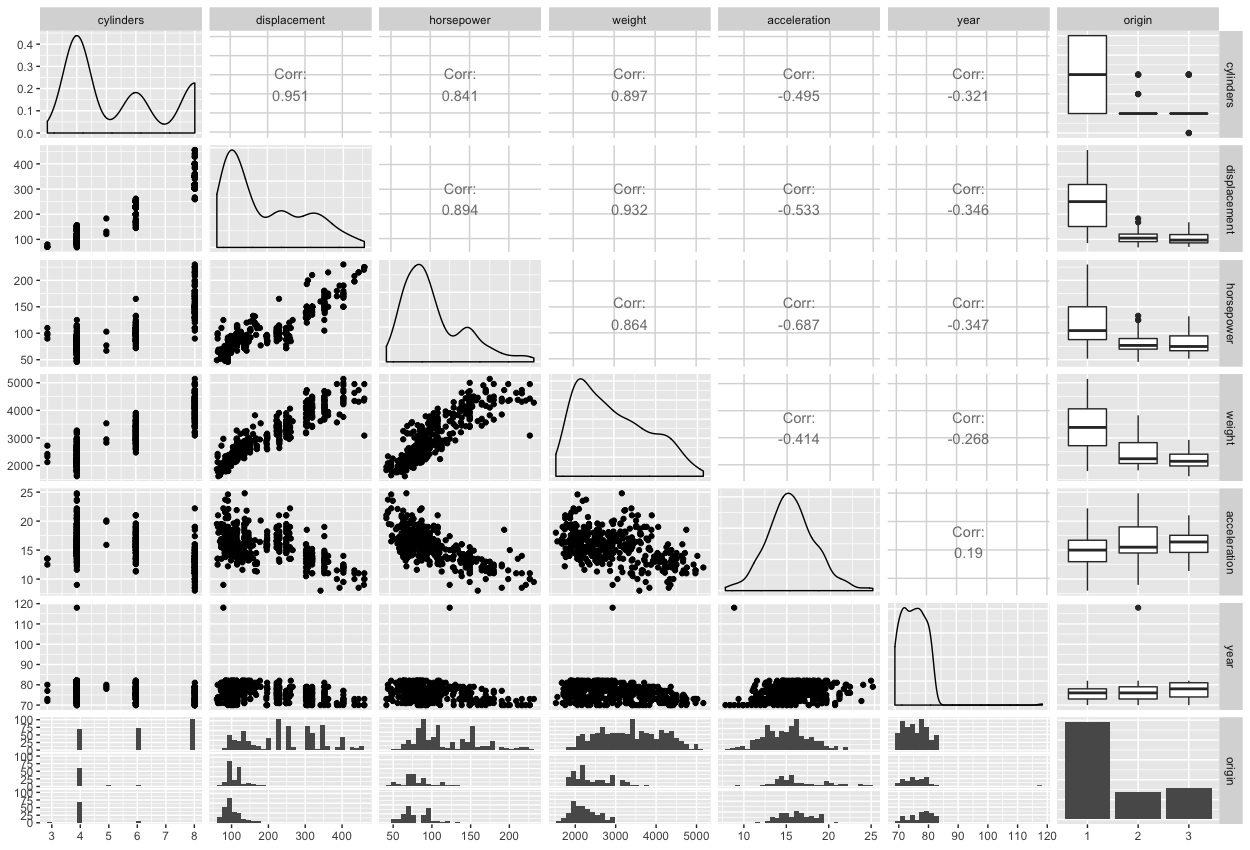
\includegraphics[scale=0.3]{pair_cor}
\end{center}
From this, it shows the offending variable with high correlation is cylinder, displacement, horsepower and weight. This makes sense since if you have a heavy car you will need more horsepower, more horsepower means more or biggest cylinders which mean higher displacement. Now consider that cylinder, displacement, horsepower and weight is combined into one in the form of:
$$
x'=\frac{cylinder+weight}{horsepower+displacement}
$$
The reason for this is that the output of this need to be reasonable, $x'$ could have been the product of all the variable but that will give it a large value and therefore when calculating the variance the inverse will be small and hence give large conditional indices.\\
Therefore the conditional indices are:
$$
1 ,680,3522
$$
And Eigenvector is:
$$
\begin{pmatrix}
-0.1&-0.5&0.9\\
-0.2&-0.8&-0.5\\
-1.0&0.2&0.0
\end{pmatrix}
$$
Additionally, the VIF (variance inflation factor) shows:
\begin{lstlisting}
  Variables      VIF
1     prime 3.211425
2   acceler 2.060063
3      year 1.184508
4    Origin 1.626321
\end{lstlisting}
Even though one of the conditional indices $>1000$ we can ignore since all the VIF $<4$. Therefore we can conclude the data is much less collinear than before.
%The remedies for this is to combine those variables into one:
%$$
%x'=\frac{x_1+x_2}{x_3}
%$$
%Where $x_1,x_2,x_3$ is displacement, horsepower and year respectively.
%\section{Models}
%In this section a model will be created and incrementally improve upon until it follows the assumption of the model and is a good model for the predictor.

\subsection{Base Model}
This model is fitted with no transformation, interaction and with every variable and factors. Let's see the diagnostics plot to observe whether or not this has violated our assumption.
\begin{center}
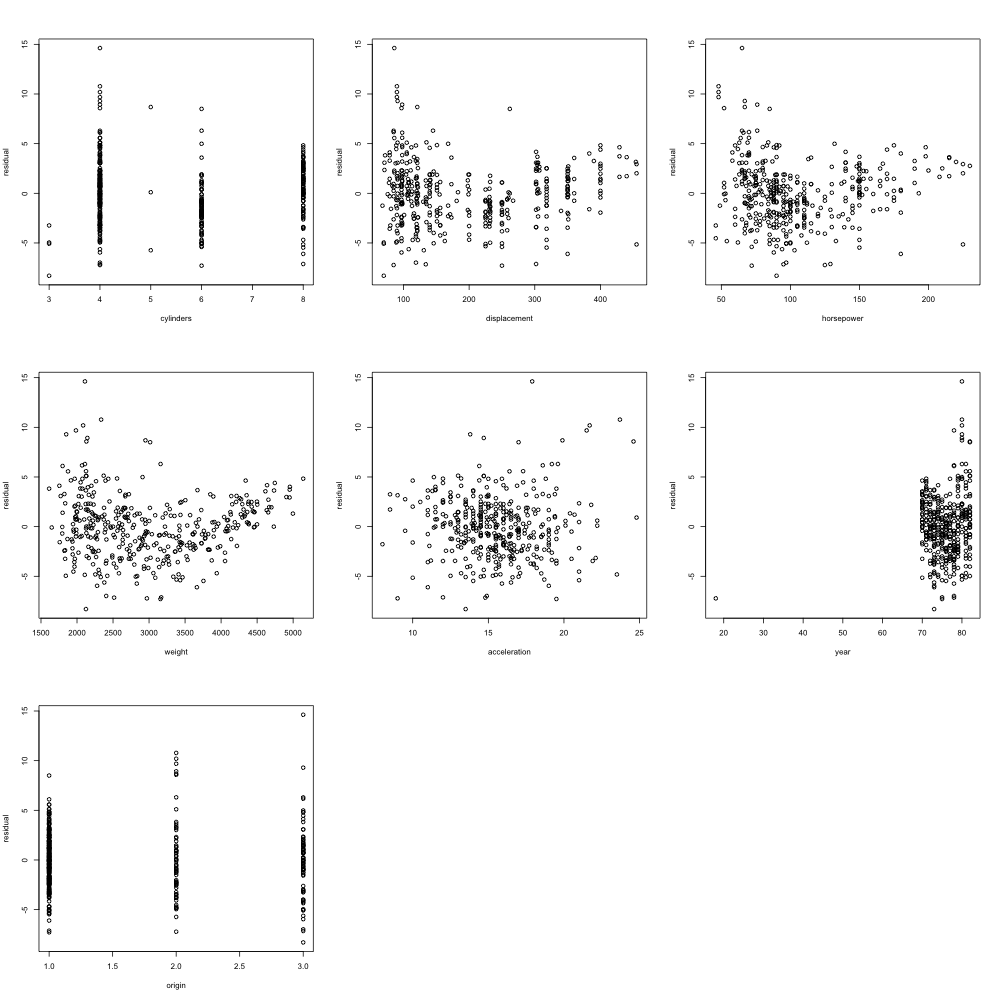
\includegraphics[scale=0.13]{1_res_vs_value}
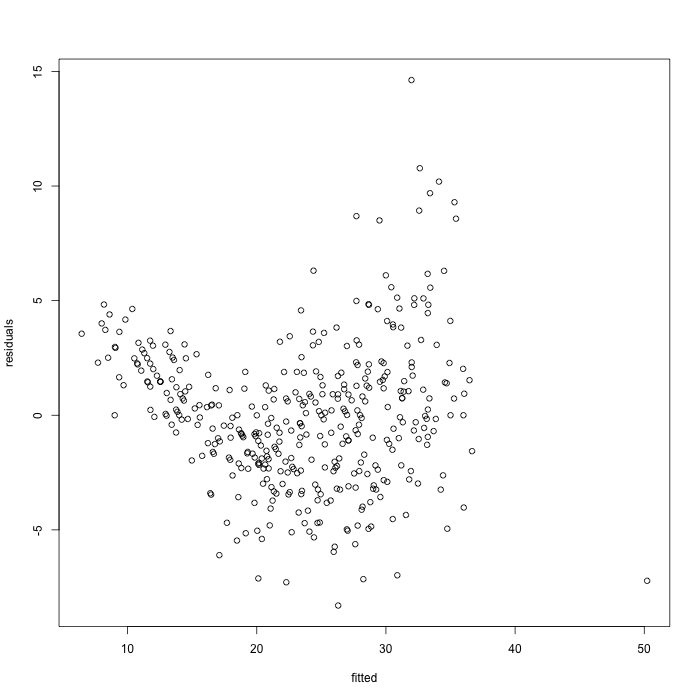
\includegraphics[scale=0.2]{1_res_vs_fitted}
\end{center}
\begin{center}
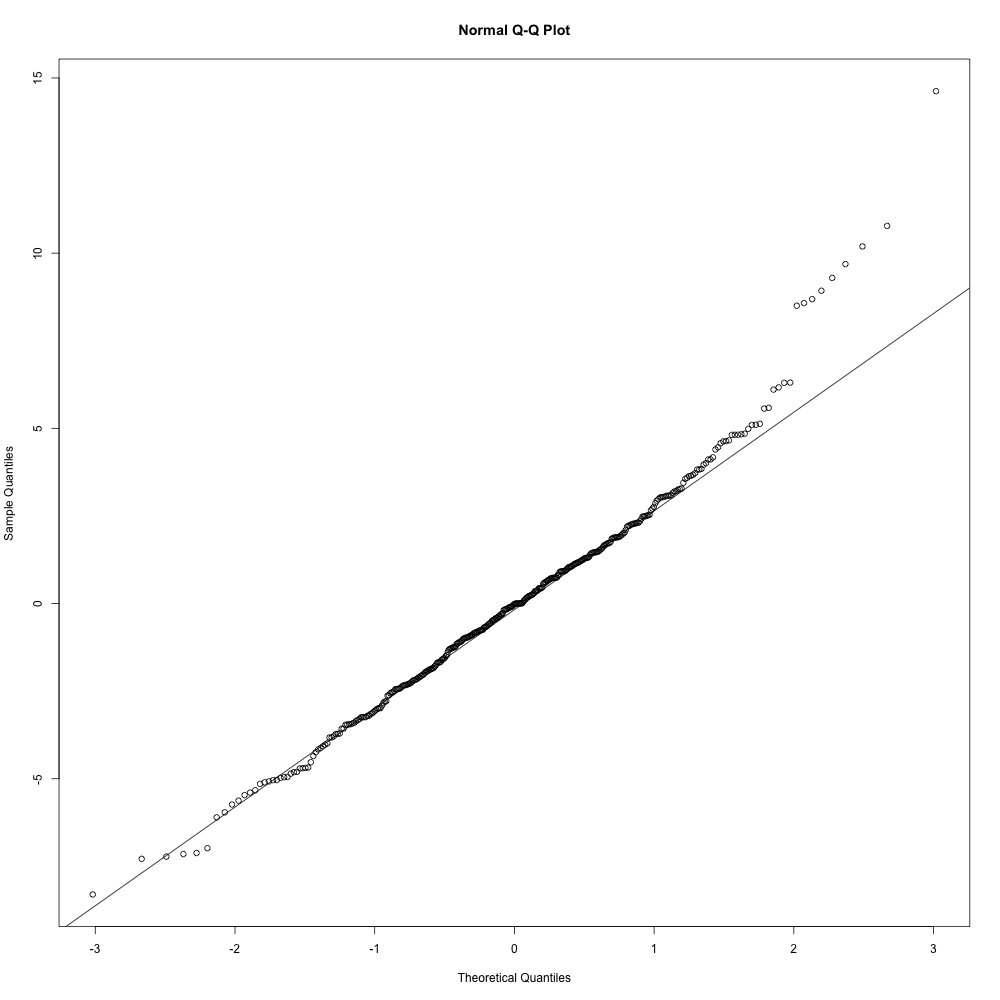
\includegraphics[scale=0.13]{1_QQplot}
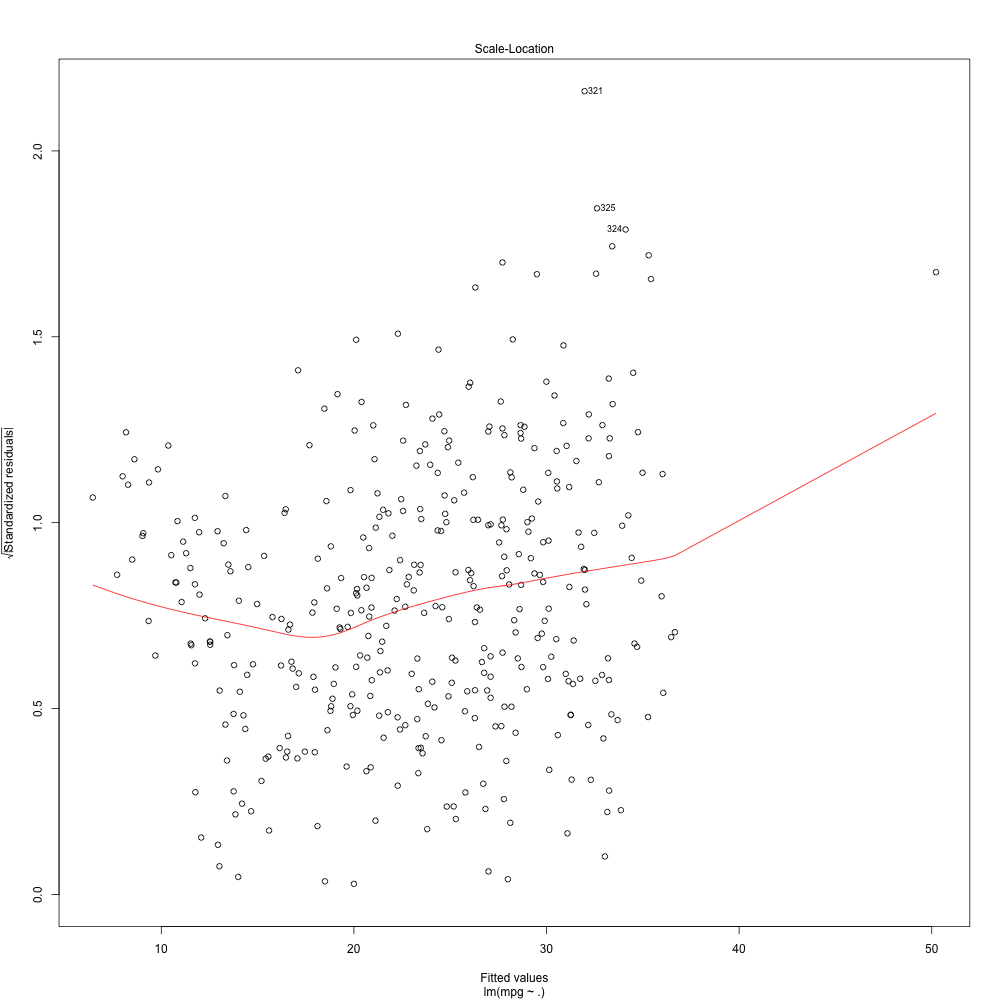
\includegraphics[scale=0.13]{1_Variance}
\end{center}
From the residual vs fitted (top right), the plot shows a none linear trends this implies a transformation is needed to make the response variable(mpg) to be linear.\\
The top right graph which is residual vs fitted we can observe a none-horizontal line across zero. Therefore this may also imply that a stabilizing variance transformation of the mpg is needed.\\
The multiple plots(top left) suggest some of the variable used is not linear. Specifically, this suggests displacement, horsepower and weight are not linear. There could also be more.\\
The Q-Q plots(bottom left) seems mostly fine apart from the upper quartile where values deviate from the line drastically. This may pose a problem later on.



%\subsection{Reciprocal of Explainatory Variable Models}
%The model for this states:
%$$
%mpg = \beta_0 +\frac{\beta_1}{displacement} + \frac{\beta_2}{weight} + \frac{\beta_2}{horse power} + ...
%$$
%The variables displacement, horsepower and weight are assign the reciprocal of it's value. If the model is now fitted around the data the plot obtain to check the assumption of model is:
%\begin{center}
%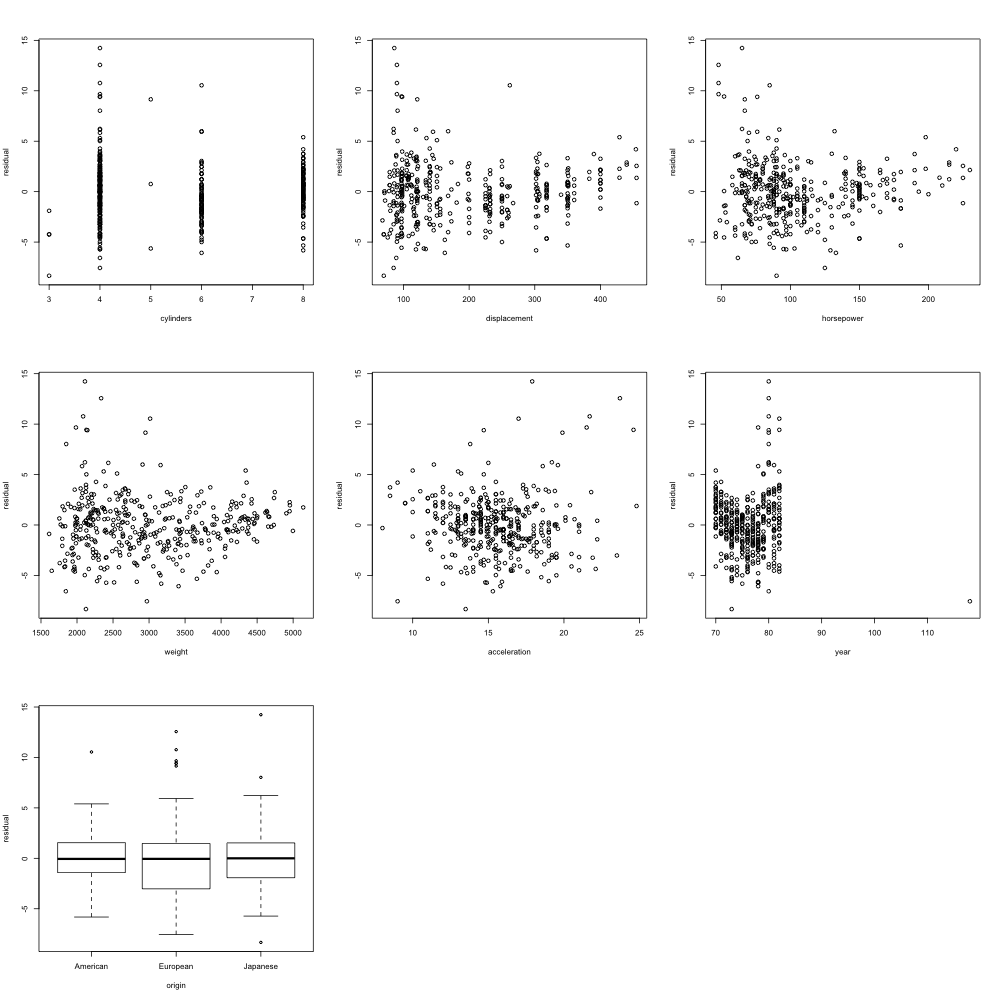
\includegraphics[scale=0.13]{model1_res_vs_value}
%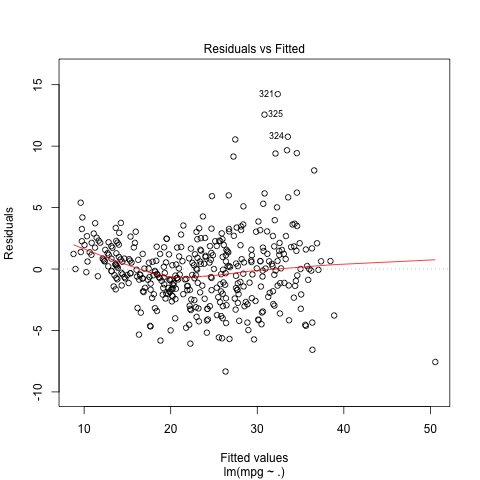
\includegraphics[scale=0.3]{model1_res_vs_fitted}
%\end{center}
%\begin{center}
%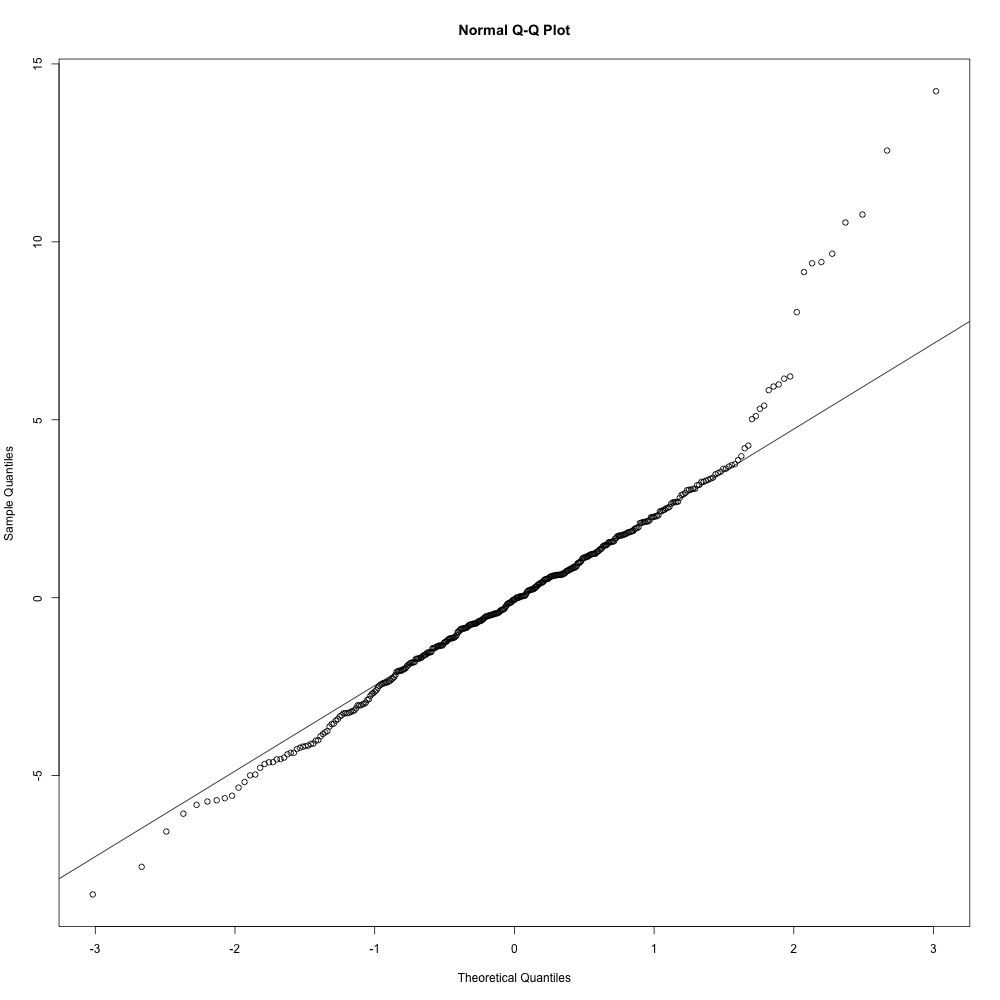
\includegraphics[scale=0.13]{model1_QQplot}
%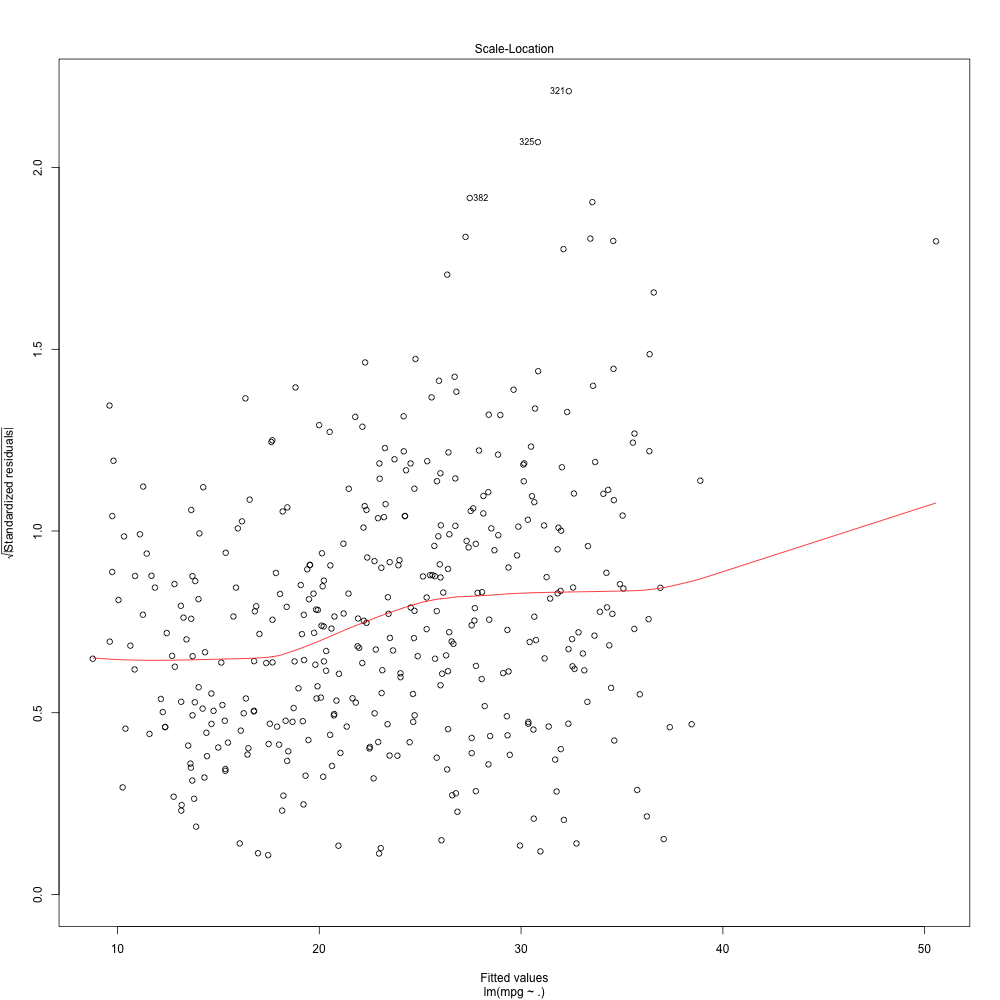
\includegraphics[scale=0.13]{model1_Variance}
%\end{center}
%The diagnostics plots tells us the transformation of the reciprocal of the variable stated above doesn't change the linearity of the model or improve the homoscedacity(bottom right plot) and it's made the normality of the model even worse (bottom right). Therefore we don't use this transformation. This model have also made the normality worse. Therefore this model is unlikely to be use for the final model.\\
%NOTE: the residual vs year is different from previous model because I've changed it so the x-axis starts at 70 rather than 0.
%\subsection{Square Root Model}
%This model states:
%$$
%\sqrt{mpg}=\beta_0+.....
%$$
%Consider a square root transformation of the model where our responds is the square root then:
%\begin{center}
%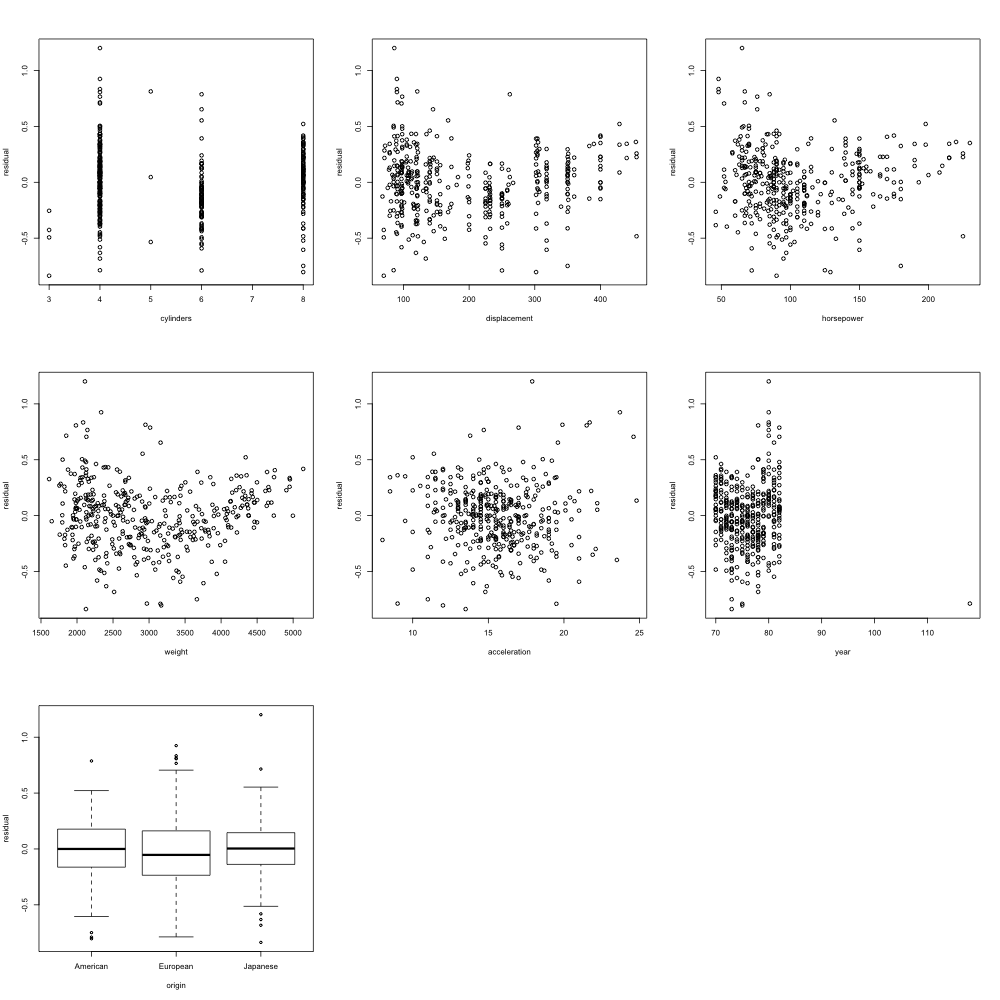
\includegraphics[scale=0.13]{sqrt_res_vs_value}
%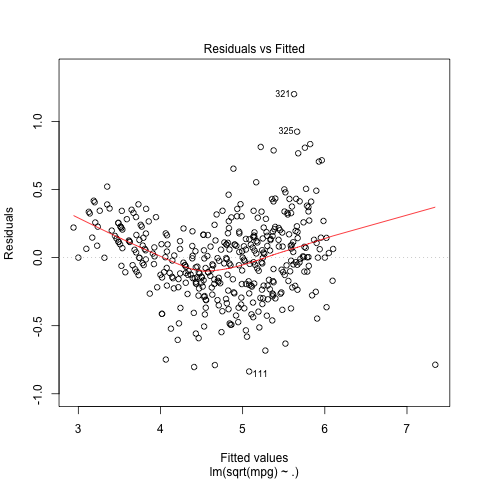
\includegraphics[scale=0.3]{sqrt_res_vs_fitted}
%\end{center}
%\begin{center}
%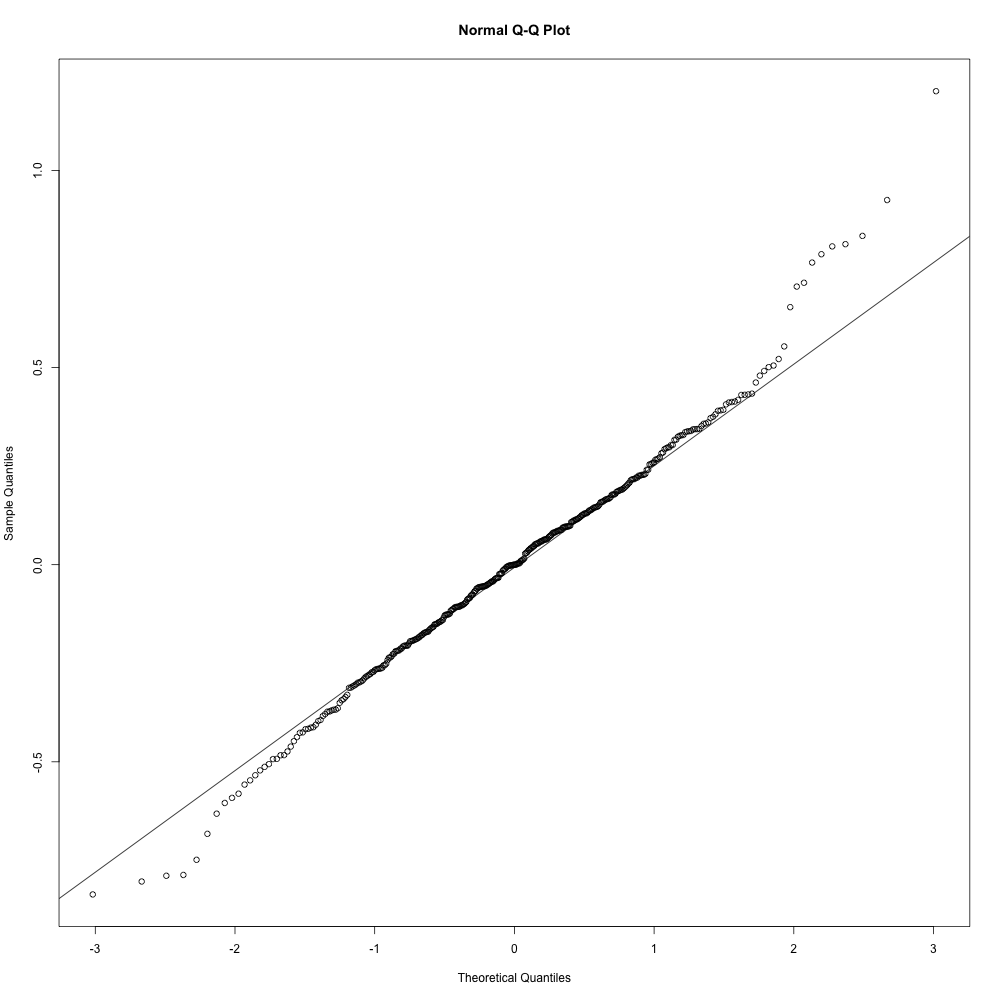
\includegraphics[scale=0.13]{sqrt_QQplot}
%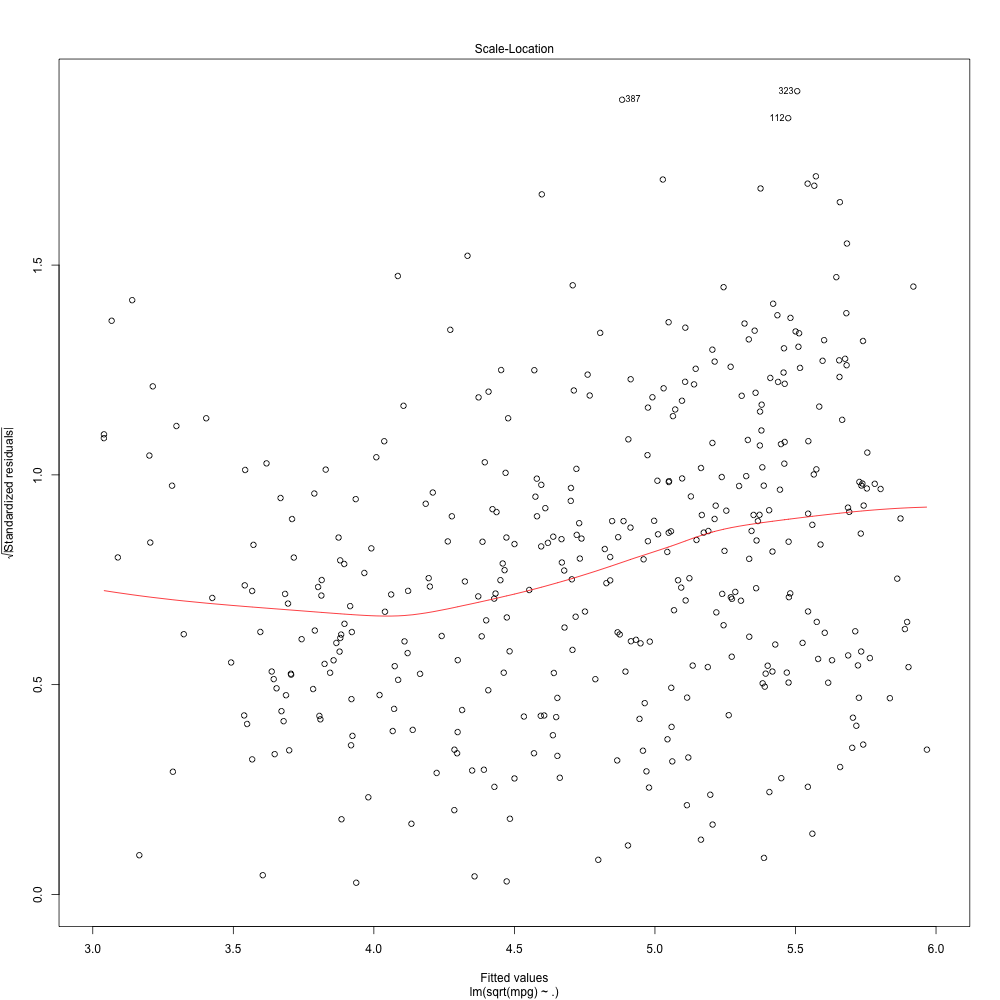
\includegraphics[scale=0.13]{sqrt_Variance}
%\end{center}
%This model is slightly better than the previous one. The residual vs fitted shows a slight none linear relationship between residual and fitted. Therefore further transformation to mpg might be needed. Similarly the there could transformation needed for the explainatory variable since the top left plot show a funnel shape behaviour between residual vs displacement, horse power and weight. Futher more they shape of the plot looks very similar, could suggest collinearity between those variables, as previous shown from the Multicollinearity analysis.


\subsection{Logarithmic Transformation}
This model is in the form of:
$$
log(mpg)= \beta_0 +.....
$$
The model in this have been fitted such that it's the logarithmic of the responds variable. The diagnostic plots shows:
\begin{center}
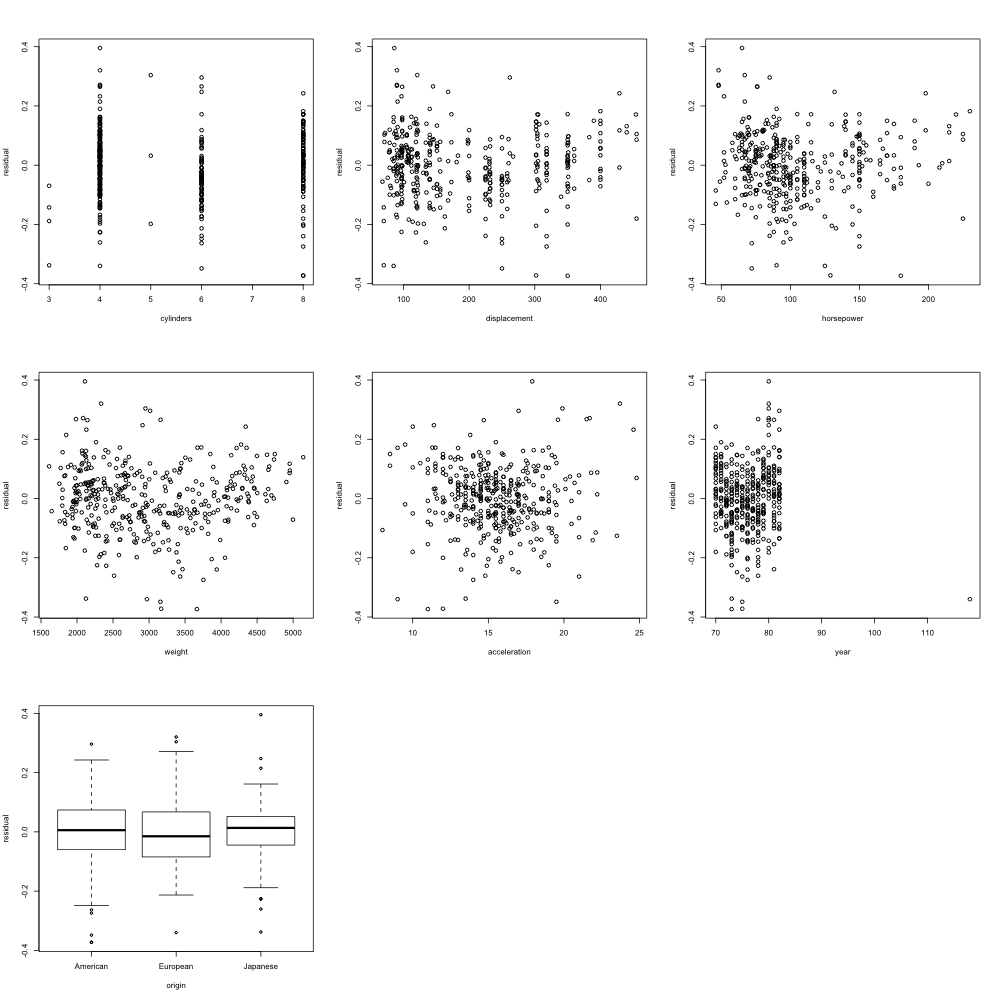
\includegraphics[scale=0.13]{3_res_vs_value}
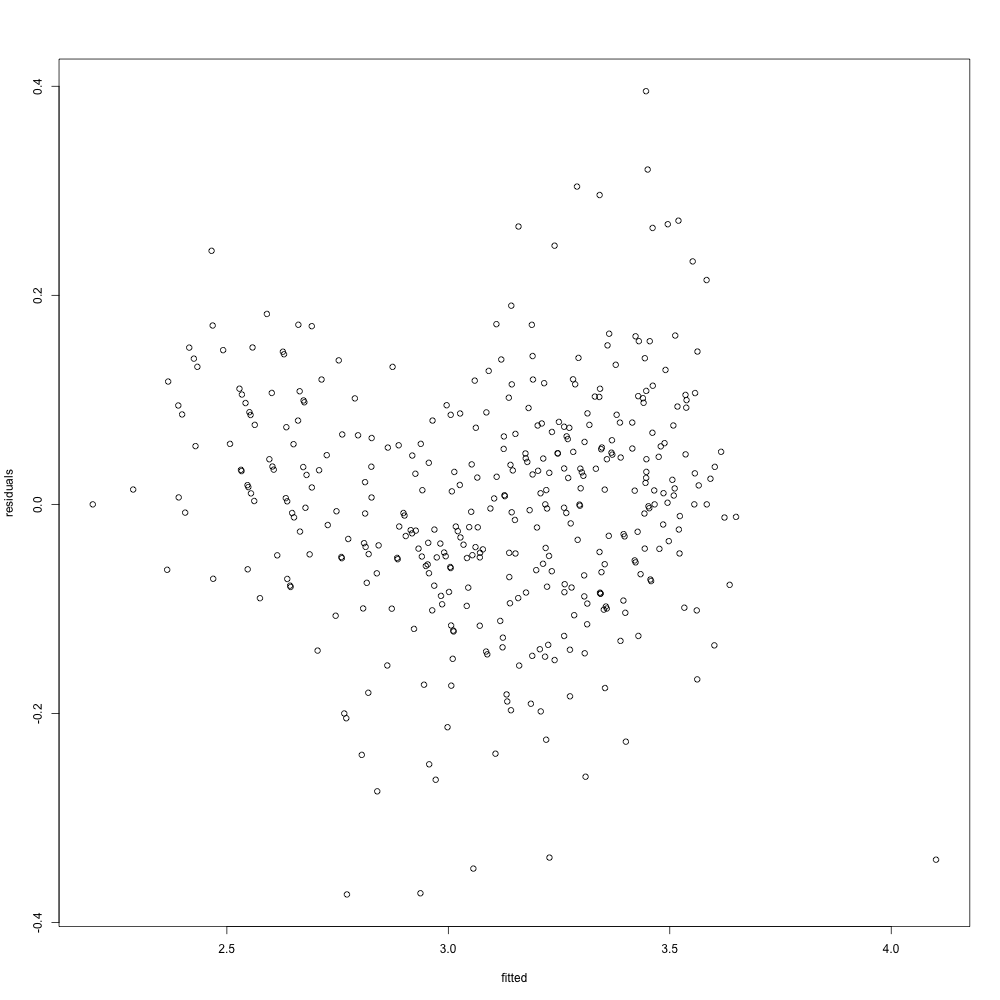
\includegraphics[scale=0.13]{3_res_vs_fitted}
\end{center}
\begin{center}
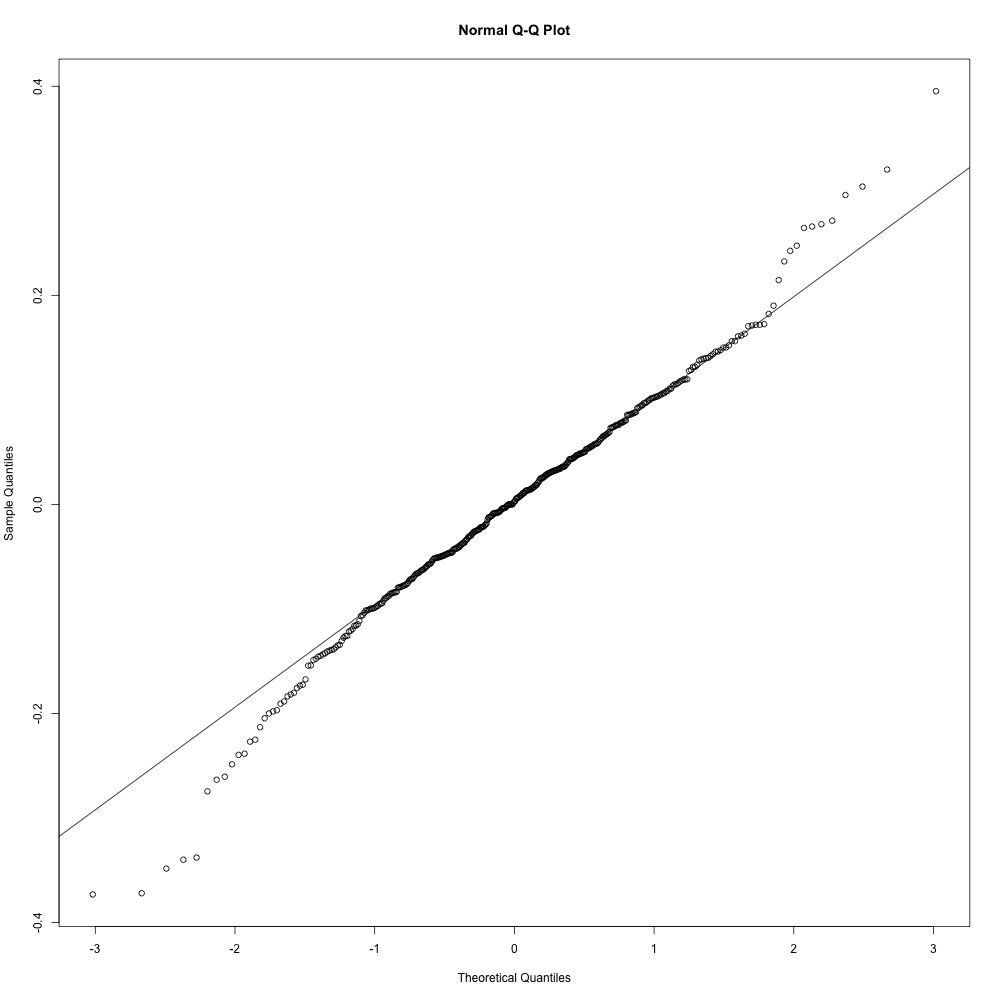
\includegraphics[scale=0.13]{3_QQplot}
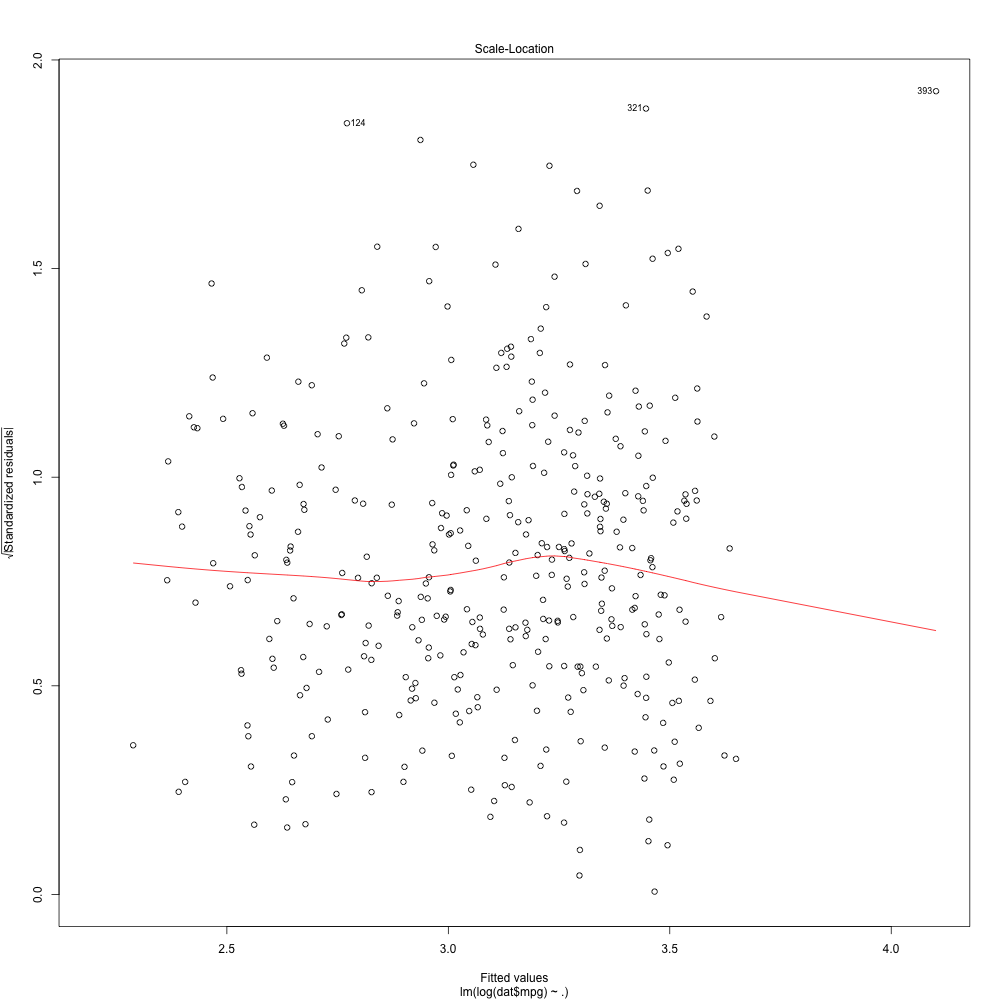
\includegraphics[scale=0.13]{3_Variance}
\end{center}
This is a relatively good transformation. The residual vs explainatory variable(top left) tells us the model now is more linear than it was before.


\subsection{Reciprocal Transformation}
This model is in the form of:
$$
\frac{1}{mpg}= \beta_0 + ....
$$
The model in this have been fitted such that it's the reciprocal of the responds variable. The diagnostic plots shows:
\begin{center}
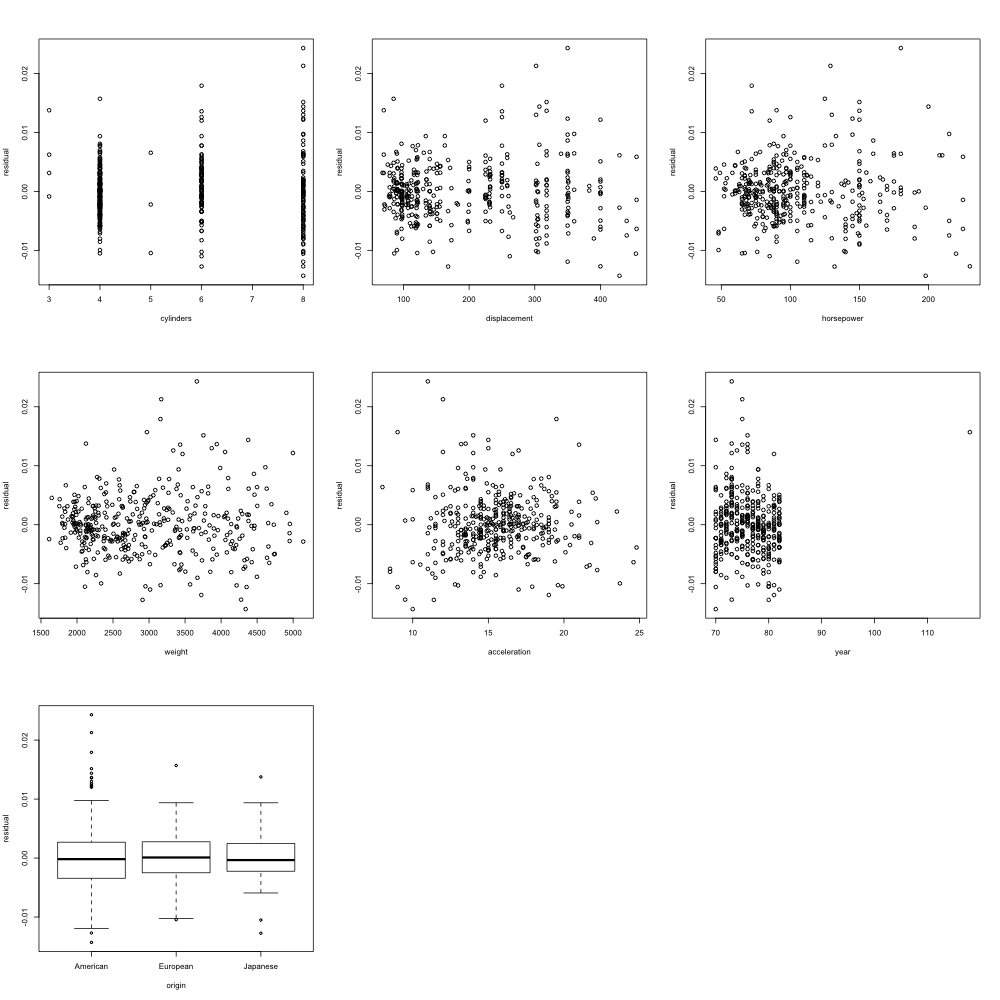
\includegraphics[scale=0.13]{4_res_vs_value}
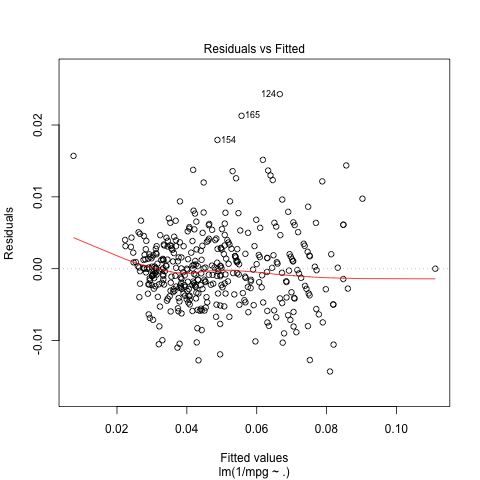
\includegraphics[scale=0.3]{4_res_vs_fitted}
\end{center}
\begin{center}
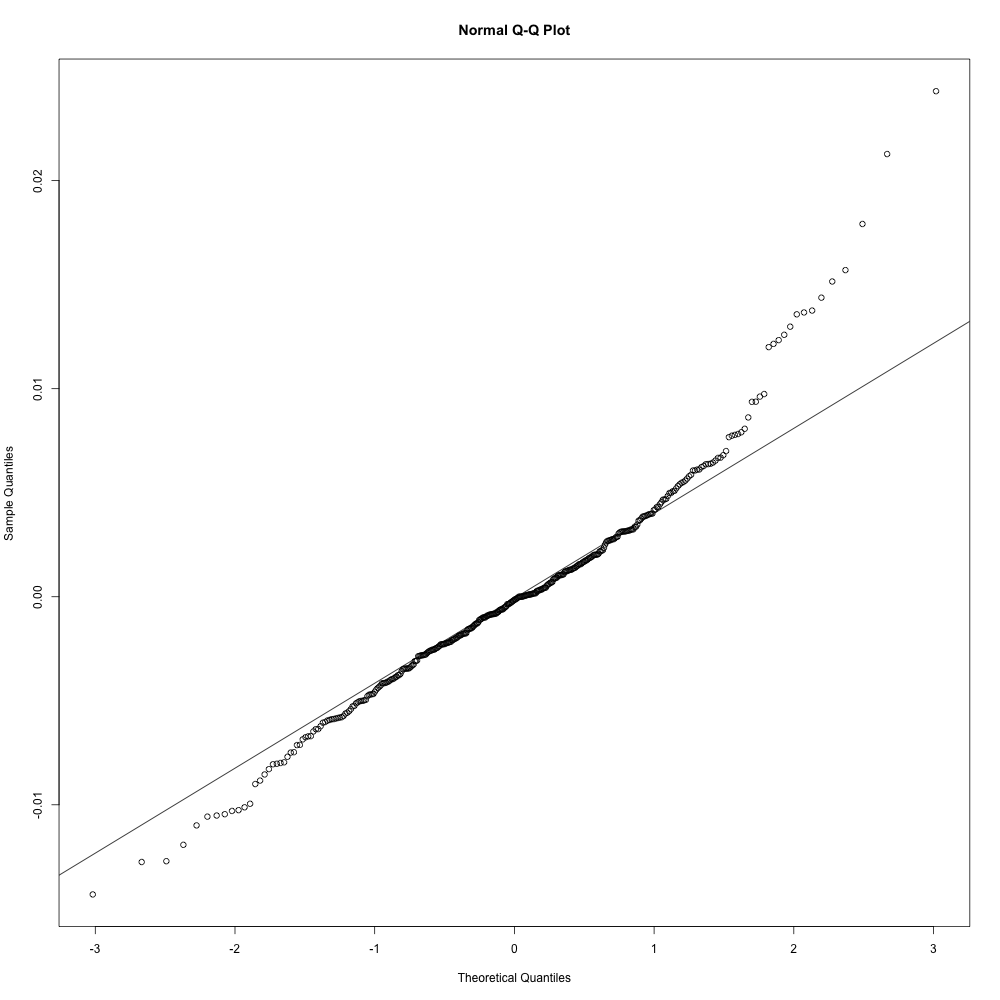
\includegraphics[scale=0.13]{4_QQplot}
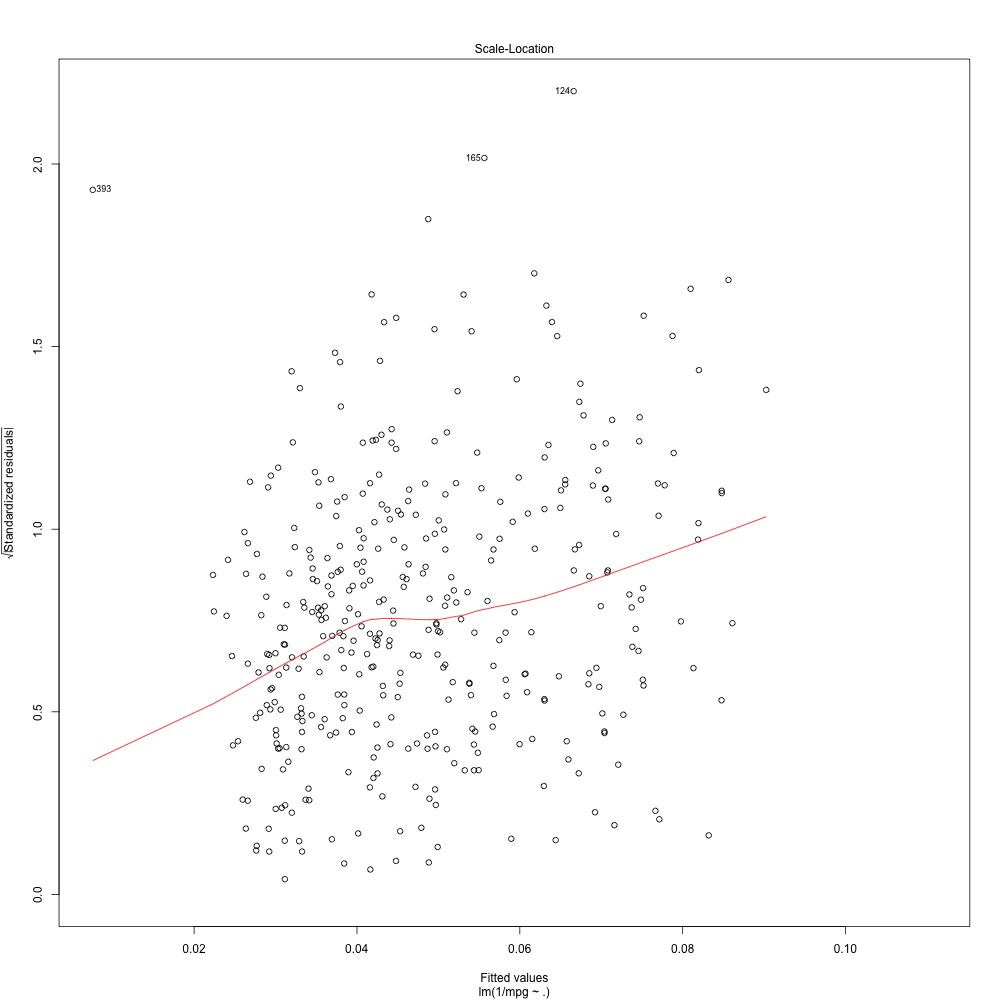
\includegraphics[scale=0.13]{4_Variance}
\end{center}
This model seems to be good for linearity of the model as shown by the explainatory variable(top left) to be more spread out and doesn't have a funnel shape as previous plots. Similarly the same can be said for the residual vs fitted plot. The problem is that this model have made the homoscedacity worse and normality of this model is slightly worse than our original model.

\subsection{Log-Reciprocal model}
This model we perform a transformation of mpg to reciprocal of that then transform it again into a logarithmic reciprocal of the mpg.
\begin{center}
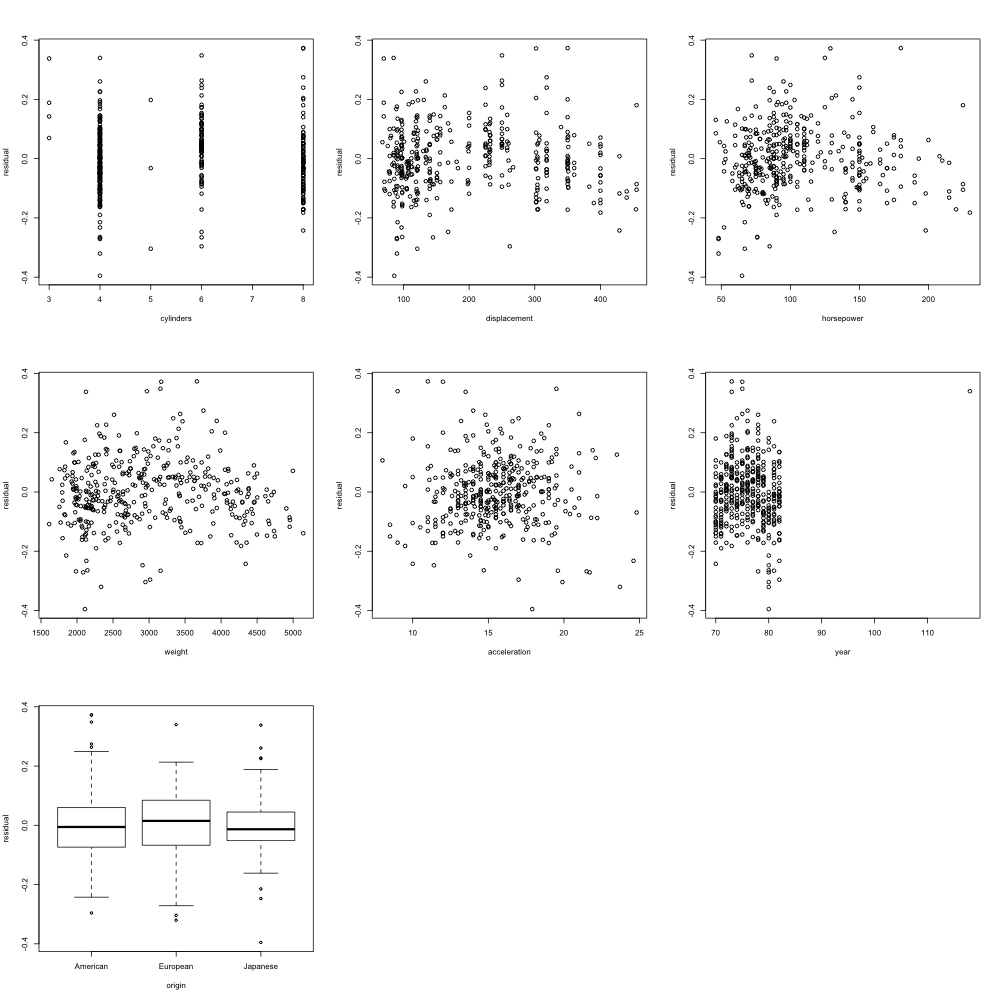
\includegraphics[scale=0.13]{5_res_vs_value}
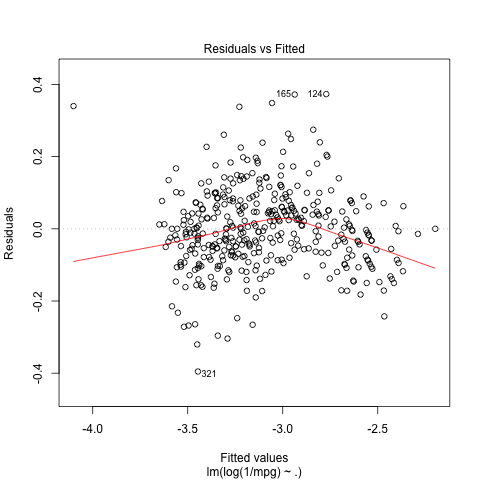
\includegraphics[scale=0.3]{5_res_vs_fitted}
\end{center}
\begin{center}
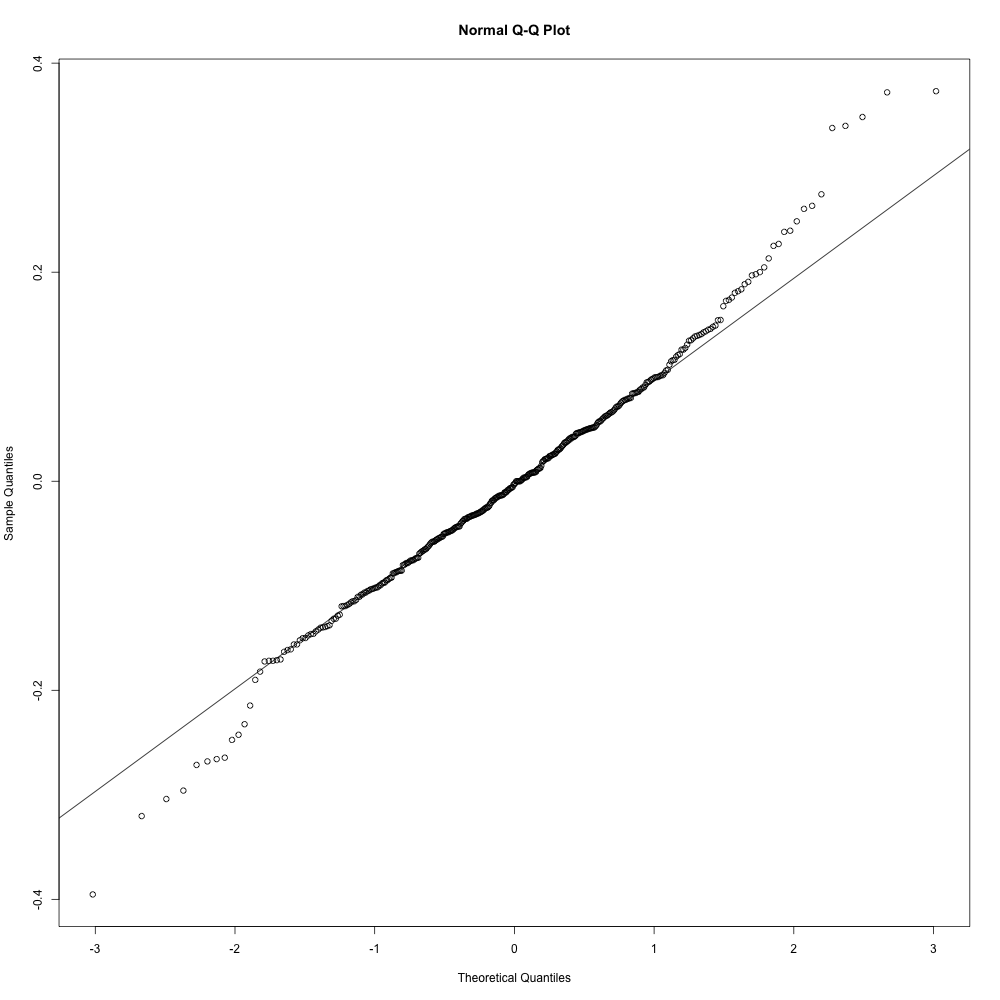
\includegraphics[scale=0.13]{5_QQplot}
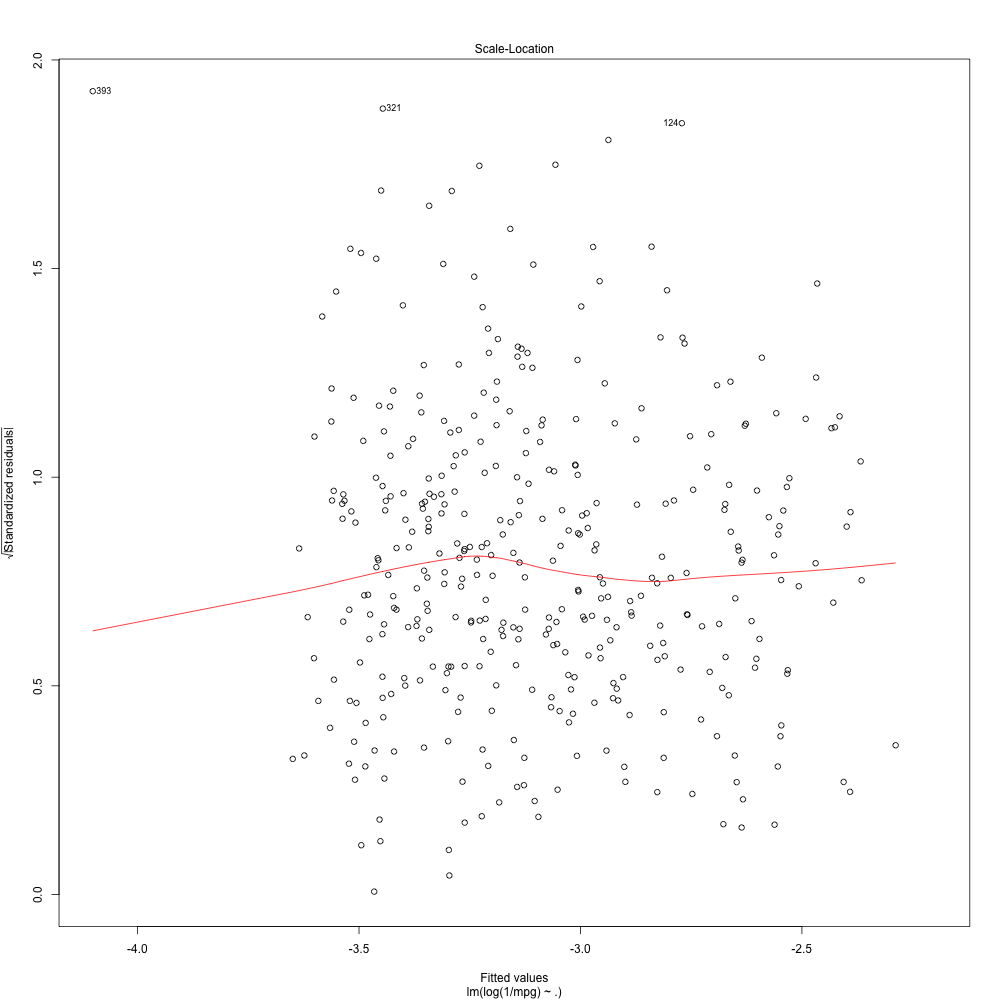
\includegraphics[scale=0.13]{5_Variance}
\end{center}
From this, we can observe that the variance is more stabilized, from the bottom right plot, from the logarithmic transformation compared to the reciprocal model. The linearity of the model (top right plot) is roughly the same as the reciprocal model, it's not a straight line but it fairs better than the square root transformation or the base model. The normality has improved from the reciprocal model (q-q plot, bottom left). Therefore this model is a good model compared to all the previous model.

%\subsection{Box-Cox Transformation}
%Since our response (mpg) is positive then the Box-Cox transformation is appropriate. Running the R-code gives us this interval for the lambda values:
%\begin{center}
%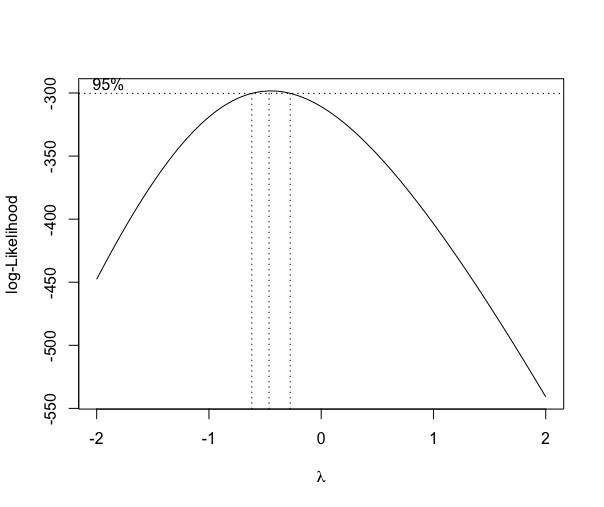
\includegraphics[scale=0.3]{boxcox}
%\end{center}
%Therefore the best suggestion for a lambda value is $\lambda = -0.5$ this mean the model is:
%$$
%mpg^{(-0.5)}=\frac{mpg^{-0.5}-1}{-0.5*mpg^{-1.5}}
%$$
%\subsection{Ridge's Regression}
%Using the R code for Ridges regression. The lambda (k value) is very small, possibly even zero. Therefore it can be concluded that Ridge's Regression was not helpful in this scenario.
%\subsection{Selecting Model}
%An attempt was made to split the data file into two categories, one training and one testing. Unfortunately, the to run the test data to obtain how well the models perform much exceeded the stack limit of R and the amount of Ram in my computers and therefore unable to attain how well each of the models performs. The only other criteria are how well the model conforms to the assumption and the residual of the model.\\
%From the analysis of the model assumption analysis above the logarithmic 
%\textbf{Residual}
%running the R-code provide gives the value of:
%\begin{lstlisting}
%         base square root      log reciprocal   model1 log reciprocal Ridge
%[1,] 3841.958    32.73854 4.862929 0.01028882 3328.877       4.862929 33.53
%\end{lstlisting}
%From this the worse models are the base model, model1 while log and reciprocal model perform better than the rest. Therefore the model that will be chosen is reciprocal and closely followed the log model.
\subsection{Model Analysis}
An attempt was made to split the data file into two categories, one training and one testing. Unfortunately, the to run the test data to obtain how well the models perform much exceeded the stack limit of R and the amount of Ram in my computers and therefore unable to attain how well each of the models performs. The only other criteria are how well the model conforms to the assumption and the residual of the model.\\
From the analysis of the model assumption analysis above the logarithmic 
\textbf{Residual}
running the R-code provide gives the value of:
\begin{lstlisting}
         base square root      log reciprocal   model1 log reciprocal Ridge
[1,] 3841.958    32.73854 4.862929 0.01028882 3328.877       4.862929 33.53
\end{lstlisting}
From this, the worse models are the base model, model1 while log and reciprocal model perform better than the rest. Therefore the model that will be chosen is reciprocal and closely followed the log model. The summary of these model also shows that the log and reciprocal model have an Adjusted-R of about 0.65 which is good considering there AIC isn't used yet.\\
NOTE: lots more model was produced and analysed but due to space constraint was not included in the report. The model1 correspond to a naive attempt where $mpg =\beta_0 \frac{\beta_1}{cylinder}+\frac{\beta_2}{displacement}+\frac{\beta_3}{horsepower}+...$ while Ridge regression was not included due to the fact that it produce very small $k$ values suggesting a lot of the parameters should be zero.
\section{Influential Values (Outliers)}
By checking the Cook's distance the outlier will be shown and subsequently remove. Using the R-code from the Diagnostics R-code section the two model shows that the value:
\begin{lstlisting}
29, 183, 333, 375 
\end{lstlisting}
Both of the models agree which observation should be removed.
Clearly these model affect the parameters so much that these values should be omitted.\\
After applying the correction to collinearity there seems to be an extra outlier namely 393 which correspond to the 2018 car. Therefore remove that data too.
\section{Variables Selection for Models}
Using AIC(Akaike information criterion) the model can be reduced down including all of its interactions. Unfortunately, due to the solution of solving the multicollinearity, it has seemed to make it so the AIC can't perform the variable reduction if the interaction is included. Therefore these model will not include interaction.\\
When AIC is performed on both of these models without interaction the model shows that acceleration is not needed. Therefore the final coefficient for the model is:
\begin{lstlisting}
#Logarithmic model

# Call:
#   lm(formula = log(mpg) ~ prime + year + origin, data = dat3)
# 
# Coefficients:
#   (Intercept)        prime         year       origin  
# 0.11322      0.08052      0.02581      0.09420  

#Reciprocal Model

#   lm(formula = 1/mpg ~ prime + year + origin, data = dat3)
# 
# Coefficients:
#   (Intercept)        prime         year       origin  
# 0.185501    -0.004119    -0.001142    -0.003869  
\end{lstlisting}
The AIC for the logarithmic model is $-1276.9$ while reciprocal is $-3609.66$. Which shows the logarithmic model is much better, but this is false as shown in the next section.


\section{Interpretation of Model}
The model that is going to be used is the exponential model in the form of:
$$
mpg = e^{0.08052*\frac{cylinder+weight}{horsepower + displacement}}*e^{0.02581*year}*e^{0.0942*origin}
$$
The intuition behind this model is that the increase in horsepower and displacement decrease the mpg exponentially while keeping the other variables constant. The year also factor into this model in an intuitive way, the newer the car the higher the mpg; which is a reasonable trend. Similarly for the origin, since Japan is numerical equivalent to 3 then under our model Japanese car would have the higher mpg while American car would have the lower mpg.
\section{Predicting Values}
We are given Japanese manufactured (in 2000) car, which has weight 2734 lbs, engine displaces- meant 81 ins3, horsepower 101 hp, 4 cylinders, and acceleration (0–60) is 12.6 seconds. The prediction is:
\begin{lstlisting}
# fit      lwr      upr
# 1 4.187991 4.074648 4.301334
\end{lstlisting}
Therefore the mpg for this car would be $e^{4.074}=58.8\geq mpg\geq 73.8 = e^{4.30134}$ with the fitted value landing round about 65.89 mpg.
\section{Summary and Reflection}
There were a few problems such as fitting the model before solving the multicollinearity problem to check the assumption then revisiting to re-check the model assumptions. The second problem is that I should have used $\frac{1}{cylinder+weight+horspower+displacement}$ as the new prime variable since this would make a better explanation of why the mpg decrease and those variable increase. For the prediction section, unfortunately, the reason why the reciprocal model performs so well, in the sense of having small residual, is because it produces a large range of confidence interval for instance if the reciprocal model was used th predict the value above it would yield:
\begin{lstlisting}
# fit          lwr         upr
# 1 -0.002286896 -0.008114051 0.003540259
\end{lstlisting}
Which implies that our mpg is between $282.27 \geq mpg$ which is very large and not right. Which means this model is not good for prediction.\\
\textbf{The r-code for this can be found on my github under `Rcode.r`}
\newpage
\section{R-Code}
\subsection{Cleaning data}
\begin{lstlisting}
> dat = read.table("http://www1.maths.leeds.ac.uk/~charles/math3714/Auto.csv",
 header = T)
> View(dat)
> summary(dat)
mpg         cylinders    displacement     horsepower
Min.   : 9.0    Min.   :3.000    Min.   : 68.0     Min.   : 46.0
1st Qu.:17.0    1st Qu.:4.000    1st Qu.:105.0    1st Qu.: 75.0
Median :23.0    Median:4.000    Median :151.0    Median : 94.0
Mean   :23.5    Mean   :5.468    Mean   :194.1    Mean   :104.5
3rd Qu.:29.0    3rd Qu.:8.000    3rd Qu.:267.0    3rd Qu.:125.0
Max.   :46.6    Max.   :8.000    Max.   :455.0    Max.   :230.0

weight        acceleration    year        origin
Min.   :1613    Min.   : 8.00    Min.   :18.00    Min.   :1.000
1st Qu.:2226    1st Qu.:13.70    1st Qu.:73.00    1st Qu.:1.000
Median :2807    Median :15.50    Median :76.00    Median :1.000
Mean   :2978    Mean   :15.52    Mean   :75.83    Mean   :1.578
3rd Qu.:3613    3rd Qu.:17.00    3rd Qu.:79.00    3rd Qu.:2.000
Max.   :5140    Max.   :24.80    Max.   :82.00    Max.   :3.000

name
amc matador       :  5
ford pinto        :  5
toyota corolla    :  5
amc gremlin       :  4
amc hornet        :  4
chevrolet chevette:  4
(Other)           :366
\end{lstlisting}
\textbf{Error in Year}
\begin{lstlisting}
> dat$year[dat$name=='vw golf estate S 1.4 TSI'] = 118
> View(dat)
\end{lstlisting}
\textbf{Problems with Names}
\begin{lstlisting}
dat = read.table("http://www1.maths.leeds.ac.uk/~charles/math3714/Auto.csv", header = T, stringsAsFactors = F)
#---Addressing 2nd problem
#In order to achieved this I need to add an extra tag into the 
#dataframe which is "stringAsFactors=F".
#adding a extra entry called make which stands for the maker of the car.
dat$make = dat$name

#changing the string into the first word of the string.
#Then attaching the first word of the string to make the table.
for(string in dat$make){
  substring = strsplit(string, " ")[[1]]
  maker = substring[1]
  print(maker)
  dat$make[dat$make==string]=maker
}

#changing the string into every word apart from the first word.
for(string in dat$name){
  substring = strsplit(string, " ")[[1]]
  print(paste(substring[-1], collapse=' ' ))
  dat$name[dat$name==string]=paste(substring[-1], collapse=' ' )
}
\end{lstlisting}
\textbf{Duplication of Car Makers}
\begin{lstlisting}
>table(dat$make)
amc    audi    bmw    buick    cadillac    capri    chevroelt
27    7    2     17    2         1     1 
chevrolet    chevy    chrysler    datsun 
43        3     6         23 
dodge    fiat    ford    hi    honda    maxda    mazda
28     8    48     1    13    2    10    
mercedes mercedes-benz    mercury    nissan 
1     2        11    1 
oldsmobile    opel     peugeot    plymouth    pontiac    renault
10        4    8    31        16    3
saab    subaru    toyota    toyouta    triumph
4    4    25    1    1 
vokswagen    volkswagen     volvo    vw 
1        15        6    7 
\end{lstlisting}
\begin{lstlisting}
>dat$make = factor(dat$make)
>dat$origin[dat$origin==1]='American'
>dat$origin[dat$origin==2]='European'
>dat$origin[dat$origin==3]='Japanese'
>dat$origin = factor(dat$origin)
\end{lstlisting}
\textbf{Uniqueness of Name}
\begin{lstlisting}
#---Problem 5
dat$name=NULL
\end{lstlisting}
\textbf{Multicollinearity}
\begin{lstlisting}
> X=as.matrix(cbind(dat$cylinders,dat$displacement,dat$horsepower,
dat$weight,dat$acceleration,dat$year))
> round(diag(solve(t(X)%*%X)),3) 
[1] 0.009 0.000 0.000 0.000 0.001 0.000
> v=eigen(t(X)%*%X)
> round(v$values,1)
[1] 3791200361.7    1365742.4     130921.6      68541.8       1553.3        111.5
> round(max(v$values)/v$values,0)
[1]        1     2776    28958    55312  2440751 34013500
> round(v$vectors,1)
     [,1] [,2] [,3] [,4] [,5] [,6]
[1,]  0.0  0.0  0.0  0.0  0.0    1
[2,] -0.1 -0.9  0.0 -0.3  0.0    0
[3,]  0.0 -0.2  0.9  0.4 -0.1    0
[4,] -1.0  0.1  0.0  0.0  0.0    0
[5,]  0.0  0.1  0.0 -0.2 -1.0    0
[6,]  0.0  0.3  0.4 -0.8  0.2    0
> S=svd(X)
> S$d
[1] 61572.72417  1168.64981   361.83087   261.80486    39.41183    10.55754
> max(S$d)/S$d
[1]    1.00000   52.68706  170.16990  235.18557 1562.29040 5832.10936
#Solving MultiCollinearity
prime = (dat$cylinders+dat$weight)/(dat$horsepower+dat$displacement)
check_multicollinearity(as.data.frame(cbind(prime,dat$acceleration,dat$year)))
# [1] "Eigenvalues"
# [1] 2423800.9    3567.0     688.2
# [1] "Max Eigenvalue/Eigenvalues"
# [1]    1  680 3522
# [1] "Eigenvectors"
# [,1] [,2] [,3]
# [1,] -0.1 -0.5  0.9
# [2,] -0.2 -0.8 -0.5
# [3,] -1.0  0.2  0.0
# [1] 1556.85611   59.72403   26.23276
# [1]  1.00000 26.06750 59.34779

vif(as.data.frame(cbind(prime,dat$acceleration,dat$year)))
# Variables      VIF
# 1     prime 2.103025
# 2        V2 1.873807
# 3        V3 1.175262
\end{lstlisting}
\subsection{Models}
\textbf{First Model}
\begin{lstlisting}
#MODELS----------------------------------------------------------------------
#First function with no transformation or interactions
base_model = function(dat){
  return(lm(mpg~.,data = dat))
}

#square root model
sqrt_model = function(dat){
  return(lm(sqrt(mpg)~., data=dat))
}

#logarithmic model
log_model = function(dat){
  return(lm(log(mpg)~., data = dat))
}

recip_y = function(dat){
  return(lm(1/mpg ~., data = dat))
}

#reciprocal of certain variable
model2 = function(dat){
  dattemp=dat
  dattemp$displacement=1/dattemp$displacement
  dattemp$weight=1/dattemp$weight
  return(lm(mpg~.,data = dattemp))
}

#Ridge's Regresson
ridge=function(dat){
  library(MASS)
  return(lm.ridge(mpg~.,data = dat, lambda = seq(0, 0.000001, 0.0000001)))
}
#Box-Cox transformation
box_cox = function(dat){
  base = lm(mpg~., data = dat)
  boxcox.lm = boxcox(base)
  return(boxcox.lm)
}
\end{lstlisting}
\subsection{Diagnostics}
\begin{lstlisting}
#BENCHMARK-----------------------------------------------------------------------------
#Testing for the residual of the model
res_bench=function(dat){
  base = base_model(dat)
  square_root = sqrt_model(dat)
  Log_model = log_model(dat)
  rec_y = recip_y(dat)
  model1 = model2(dat)
  log_recip_model = lm(log(1/mpg)~., data = dat)
  LinRidge = ridge(dat)
  res_summary=cbind(sum(base$residuals^2), sum(square_root$residuals^2),sum(Log_model$residuals^2),
                    sum(rec_y$residuals^2),sum(model1$residuals^2),sum(log_recip_model$residuals^2),33.53)
  colnames(res_summary)=c("base","square root","log","reciprocal","model1", "log reciprocal","Ridge")
  print(res_summary)
}

#Diagnostics-of-Model--------------------------------------------------

#Initializing the models.
base = base_model(dat)
square_root = sqrt_model(dat)
Log_model = log_model(dat)
rec_y = recip_y(dat)
model1 = model2(dat)
log_recip_model = lm(log(1/mpg)~., data = dat)
LinRidge = ridge(dat)

#Checking the assumption of models.
check_assumption("base",base,dat)
check_assumption("model1",model1,dat)
check_assumption("sqrt",square_root,dat)
check_assumption("log",log_model,dat)
check_assumption("reciprocal",rec_y,dat)
check_assumption("log_reciprocal",log_recip_model,dat)

#Checking which model has the best residual
res_bench(dat)
# base square root     log reciprocal   model1 log reciprocal Ridge
# [1,] 8129.847    83.09975 5.60372 0.03921142 3328.877       14.86362 33.53
\end{lstlisting}
\subsection{Removing Outliers}
\begin{lstlisting}
dat = dat[-c(29,183,333,375),]
dat = dat[-393]
\end{lstlisting}

\subsection{AIC}

\begin{lstlisting}
dat3=dat2[-6]
final_log = lm(log(mpg) ~ .^2, data = dat3)
final_rec = lm(1/mpg ~ .^2, data = dat3)

#No interactions.
final_log = lm(log(mpg)~., data = dat3)
final_rec = lm(1/mpg~., data = dat3)
step(final_log, direction="both")
step(final_rec,direction = "both")
\end{lstlisting}
\subsection{Prediction}
\begin{lstlisting}
#Predicting the new value
prime = (dat$cylinders+dat$weight)/(dat$horsepower+dat$displacement)
dat2=as.data.frame(cbind(dat$mpg,prime,dat$acceleration,dat$year,dat$origin,dat$make))
colnames(dat2)=c("mpg","prime","acceleration","year","origin","make")
dat3=dat2[-6]
final_log = lm(log(mpg) ~ ., data = dat3)
final_rec = lm(1/mpg ~ ., data = dat3)
final_rec = step(final_rec,direction = "both")
summary(final_rec)
new = as.data.frame(cbind(15.043956,100,3))
colnames(new)=c("prime","year","origin")
predict.lm(final_rec,newdata=new,interval="confidence",level=0.95)
predict.lm(final_log,newdata=new, interval="confidence",level=0.95)
# fit          lwr         upr
# 1 -0.002286896 -0.008114051 0.003540259
# fit      lwr      upr
# 1 4.187991 4.074648 4.301334
\end{lstlisting}
\end{document}
